\documentclass[10pt]{beamer}

\usetheme[progressbar=frametitle]{metropolis}
\usepackage{appendixnumberbeamer}

\usepackage{booktabs}
\usepackage[scale=2]{ccicons}

\usepackage{pgfplots}
\usepgfplotslibrary{dateplot}

\usepackage{xspace}
\newcommand{\themename}{\textbf{\textsc{metropolis}}\xspace}


% ---
% PACOTES
% --
\usepackage[alf]{abntex2cite}		% Citações padrão ABNT
\usepackage[brazil]{babel}		    % Idioma do documento
\usepackage{color}			       % Controle das cores
\usepackage[T1]{fontenc}		  % Selecao de codigos de fonte.
\usepackage{graphicx}			    % Inclusão de gráficos
\usepackage[utf8]{inputenc}		   % Codificacao do documento (conversão automática dos acentos)
\usepackage{multirow}
\usepackage{threeparttable}
\usepackage[capposition=top]{floatrow}
\usepackage{txfonts}			 % Fontes virtuais
\usepackage{ragged2e}
\usepackage{etoolbox}
\usepackage{lipsum}
\usepackage{amssymb}
% ---

% ---
% Minhas Definições
% ---

%Deixando o Caption alinhado a esquerda mesmo com quebra de linha
\usepackage[labelfont=bf, justification=justified,singlelinecheck=true]{caption}


% Colocando numero de paginas no slide
\setbeamertemplate{footline}[frame number]{}
\setbeamertemplate{caption}[numbered]{}

\title{\textit{Coding Dojo} como Ferramenta para o Ensino de Programação}
\date{\today}
% \date{}
\author{Marciano Saraiva, Raul Lima e Samy Soares}
\institute{Universidade Federal do Cear\'a - Campus de Quixad\'a}
% \titlegraphic{\hfill
\includegraphics[height=1.5cm]{figuras/logo.pdf}}

\begin{document}

\maketitle

\begin{frame}{Roteiro}
  \setbeamertemplate{section in toc}[sections numbered]
  \tableofcontents[hideallsubsections]
\end{frame}

\section{Introdu\c{c}\~ao}

%% ----------------- NOVO SLIDE --------------------------------
\begin{frame}{Iniciativa}

\begin{figure}[H]
  \centering
   \begin{minipage}[b]{0.25\textwidth}\end{minipage}
  \hfill
  \begin{minipage}[b]{0.3\textwidth}
	
\includegraphics[width=\textwidth]{figuras/dojos.png}
  \end{minipage}
  \hfill
  \begin{minipage}[b]{0.1\textwidth}
    
\includegraphics[width=\textwidth]{figuras/vs.png}
  \end{minipage}
  \hfill
  \begin{minipage}[b]{0.3\textwidth}
    
\includegraphics[width=\textwidth]{figuras/petti.png}
  \end{minipage}
  \hfill
  \begin{minipage}[b]{0.25\textwidth}\end{minipage}
\end{figure}

As se\c{c}\~oes de \textit{Conding Dojos} que ocorrem na UFC - Campus Quixad\'a \'e uma iniciativa do grupo PET-Tecnologia da Informação 
e visam aprimorar as práticas de programação e a troca de conhecimento entre os seus participantes.

\end{frame}

%% ----------------- NOVO SLIDE --------------------------------
\begin{frame}{O que \'e um \textit{Coding Dojo}?}

Um \textit{Coding Dojo} é uma reunião entre desenvolvedores para aprimorar técnicas e metodologias de programação. Inspirado em fundamentos 
das artes marciais japonesas, um dojo é um local de colaboração e não de competição, onde o principal objetivo é aprender.

\end{frame}


\section{Metodologia}

%% ----------------- NOVO SLIDE --------------------------------
\begin{frame}{Metodologia}

\begin{figure}[H]
  \centering
  \begin{minipage}[b]{10cm}
	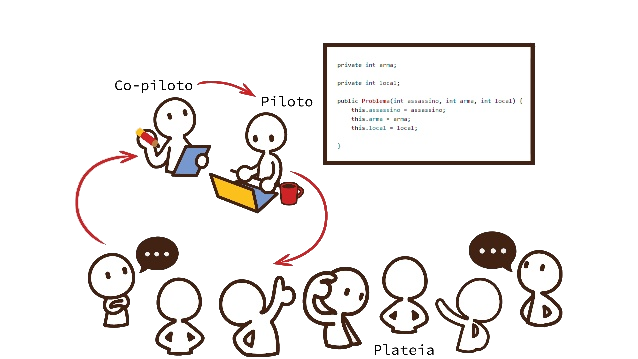
\includegraphics[width=\textwidth]{figuras/metodologia.png}
  \end{minipage}
\end{figure}

\end{frame}


%% ----------------- NOVO SLIDE --------------------------------
\begin{frame}{Metodologia}

	\begin{itemize}
		\item Programação baseada em testes
		\item Passos de bebê
		\item Programação em dupla
		\item Refatora\c{c}\~ao
		\item Propriedade Coletiva de C\'odigo
		\item Feedback
	\end{itemize}
	
\end{frame}

\section{Coding Dojos na Universidade Federal do Cear\'a}

%% ----------------- NOVO SLIDE --------------------------------
\begin{frame}{Linguagens Usadas}
	\begin{columns}
		\begin{column}{7cm}
			\begin{center}
				\vskip 0.5cm
				\Huge Manh\~a
			\end{center}
		\end{column}
		\begin{column}{7cm}
			\begin{minipage}[b]{0.4\textwidth}
				\vskip 0.5cm
				
\includegraphics[width=\textwidth]{figuras/python.png}
			\end{minipage}
		\end{column}
	\end{columns}
	\hfill
	\begin{columns}
		\begin{column}{7cm}
			\begin{center}
				\vskip 0.5cm
				\Huge Tarde
			\end{center}
		\end{column}
		\begin{column}{7cm}
			\begin{minipage}[b]{0.4\textwidth}
				\vskip 0.5cm
				
\includegraphics[width=\textwidth]{figuras/cplusplus.png}
			\end{minipage}
		\end{column}
	\end{columns}
	
\end{frame}


%% ----------------- NOVO SLIDE --------------------------------
\begin{frame}{Se\c{c}\~oes}

\begin{columns}[t]
		\begin{column}{.425\textwidth}
			\begin{block}{Se\c{c}\~oes durante as aulas}
				\begin{itemize}
					\item Realizadas conforme a disponibilidade do professor
					\item Boa participa\c{c}\~ao dos alunos
					\item Incentivo do Professor
				\end{itemize}
			\end{block}
		\end{column}
		\begin{column}{.425\textwidth}
			\begin{block}{Se\c{c}\~oes fora das aulas}
				\begin{itemize}
					\item Baixo índices de participação
					\item Impossibilidade de realizar a metodologia
				\end{itemize}
			\end{block}
		\end{column}
	\end{columns}

\end{frame}


% \section{Refer\^encias}
% ----------------- NOVO SLIDE --------------------------------
%\begin{frame}[allowframebreaks]{Refer\^encias}
%  \bibliography{demo}
%\end{frame}


\section{Coment\'arios}

% ----------------- NOVO SLIDE --------------------------------
\begin{frame}{Coment\'arios}
	\begin{columns}
		\begin{column}{2cm}
			\centering
			\vskip 0.5cm
			
\includegraphics[height=0.7\textwidth]{figuras/dojos.png}
		\end{column}
		\begin{column}{6cm}
			\centering
			\vskip 0.5cm
			\Huge Obrigado!
		\end{column}
	\end{columns}
\end{frame}



\end{document}
